\begin{appendices}
\section{}\label{sec:appendix}

\begin{figure}[h]
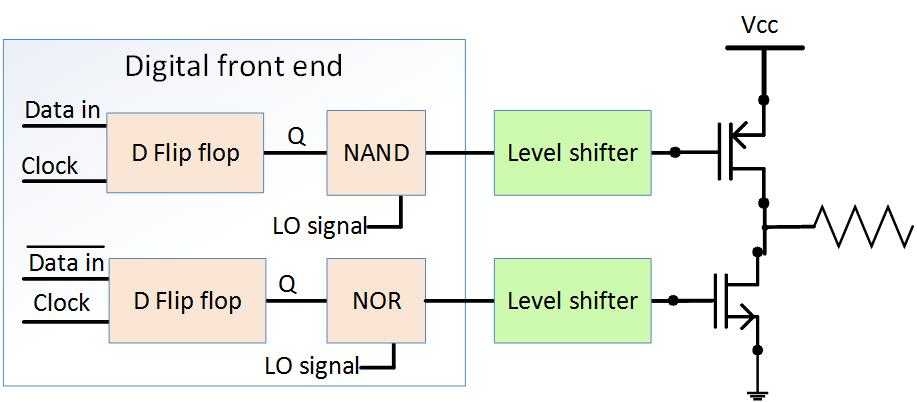
\includegraphics[width=0.5\textwidth]{Global_schematic_previous_group.jpg}
\caption{Global schematic of the previous group.~\cite{powerdac}.}
\label{fig:Global_schematic_previous_group_figure}
\end{figure}

\begin{figure}[h]
 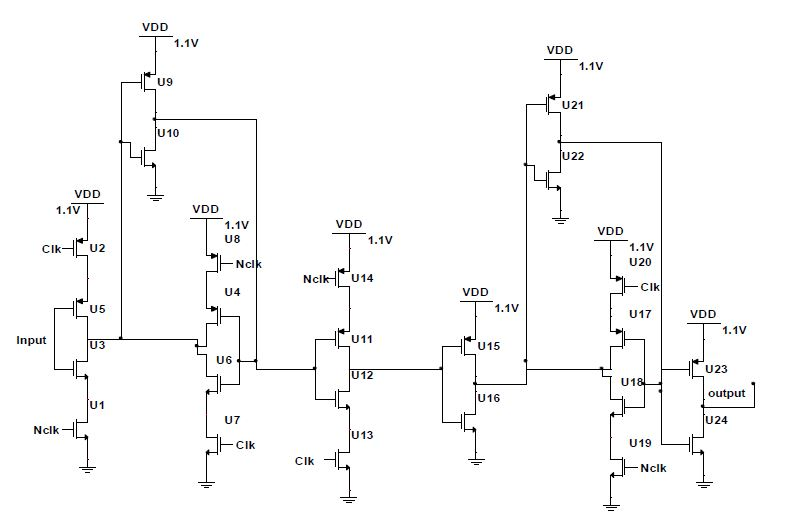
\includegraphics[width=0.5\textwidth]{D_flip_flop_schematic.jpg}
 \caption{ D flip flop schematic from previous group ~\cite{powerdac}.}
 \label{fig:D_flip_flop_ previous_group_figure}
\end{figure}

\begin{figure}[h]
 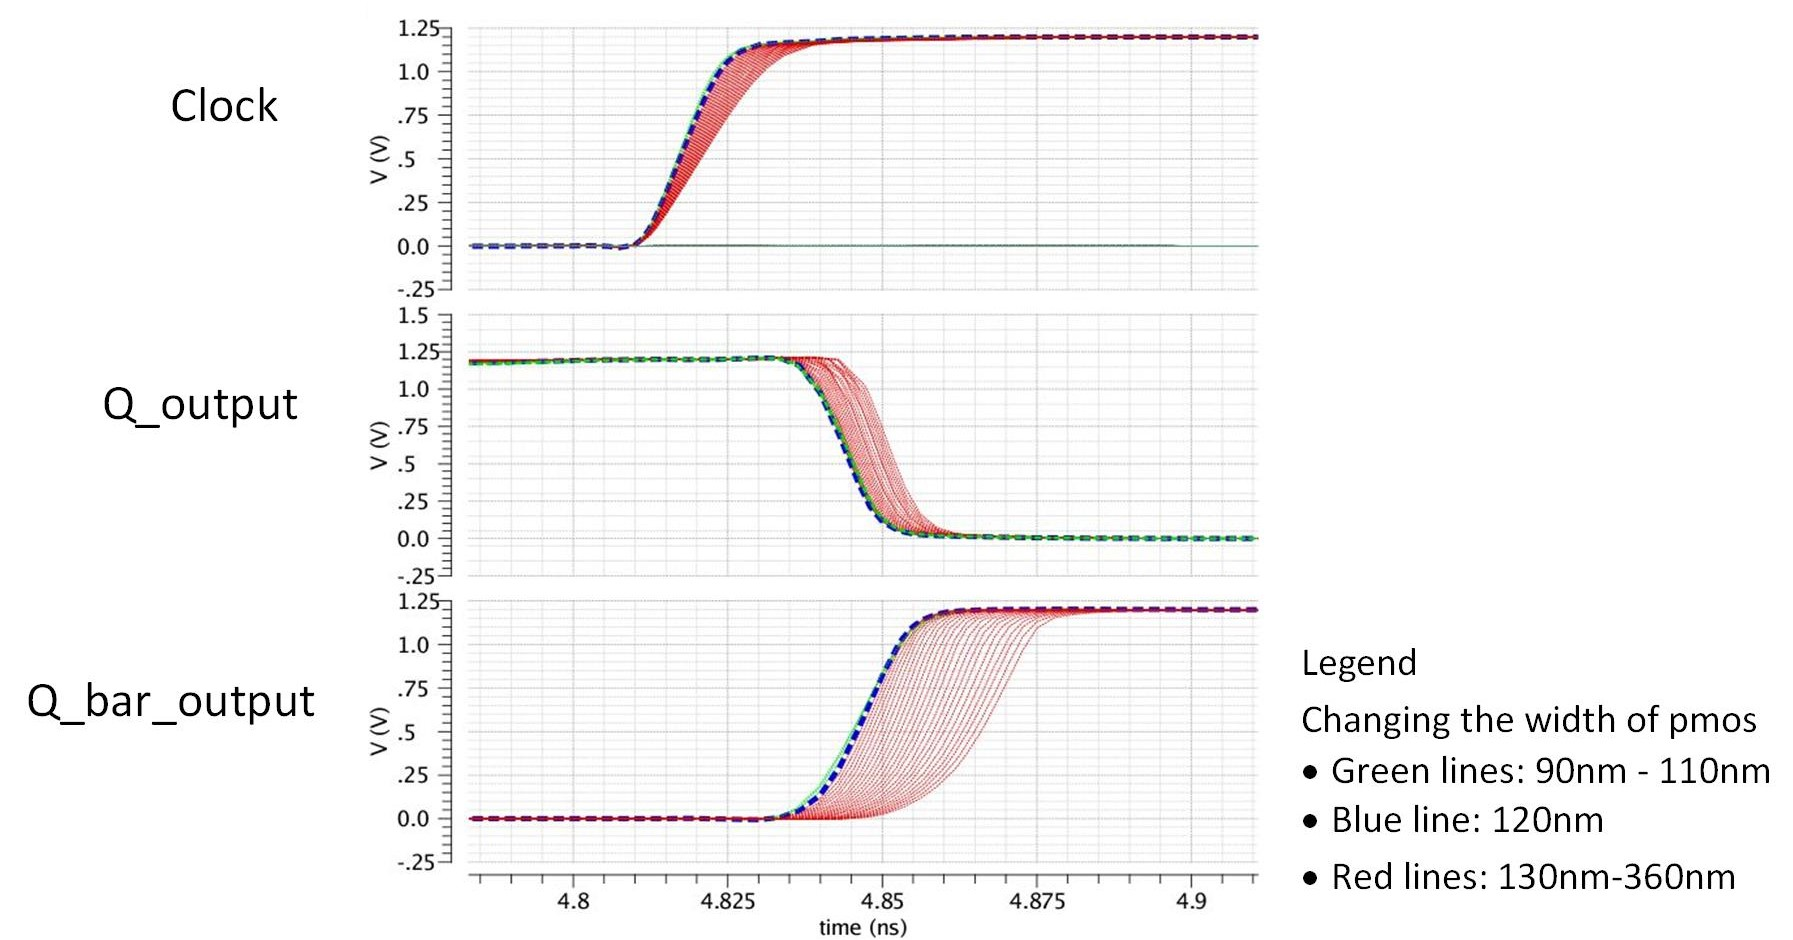
\includegraphics[width=0.5\textwidth]{Parameter_sweep_changing_w_high_to_low.jpg}
 \caption{A Parameter sweep of changing the width of the PMOS transistor when the data is low. The PMOS transistors of part 1,2 and 4 of~\ref{fig:D_flip_flop_schematic_figure} are part of the parameter sweep. The frequency of the clock is set to 1 GHz and the frequency of the data is set to 500MHz.} 
 \label{fig:parametersweep_changing_w_high_to_low_figure}
\end{figure}

\begin{figure}[h]
 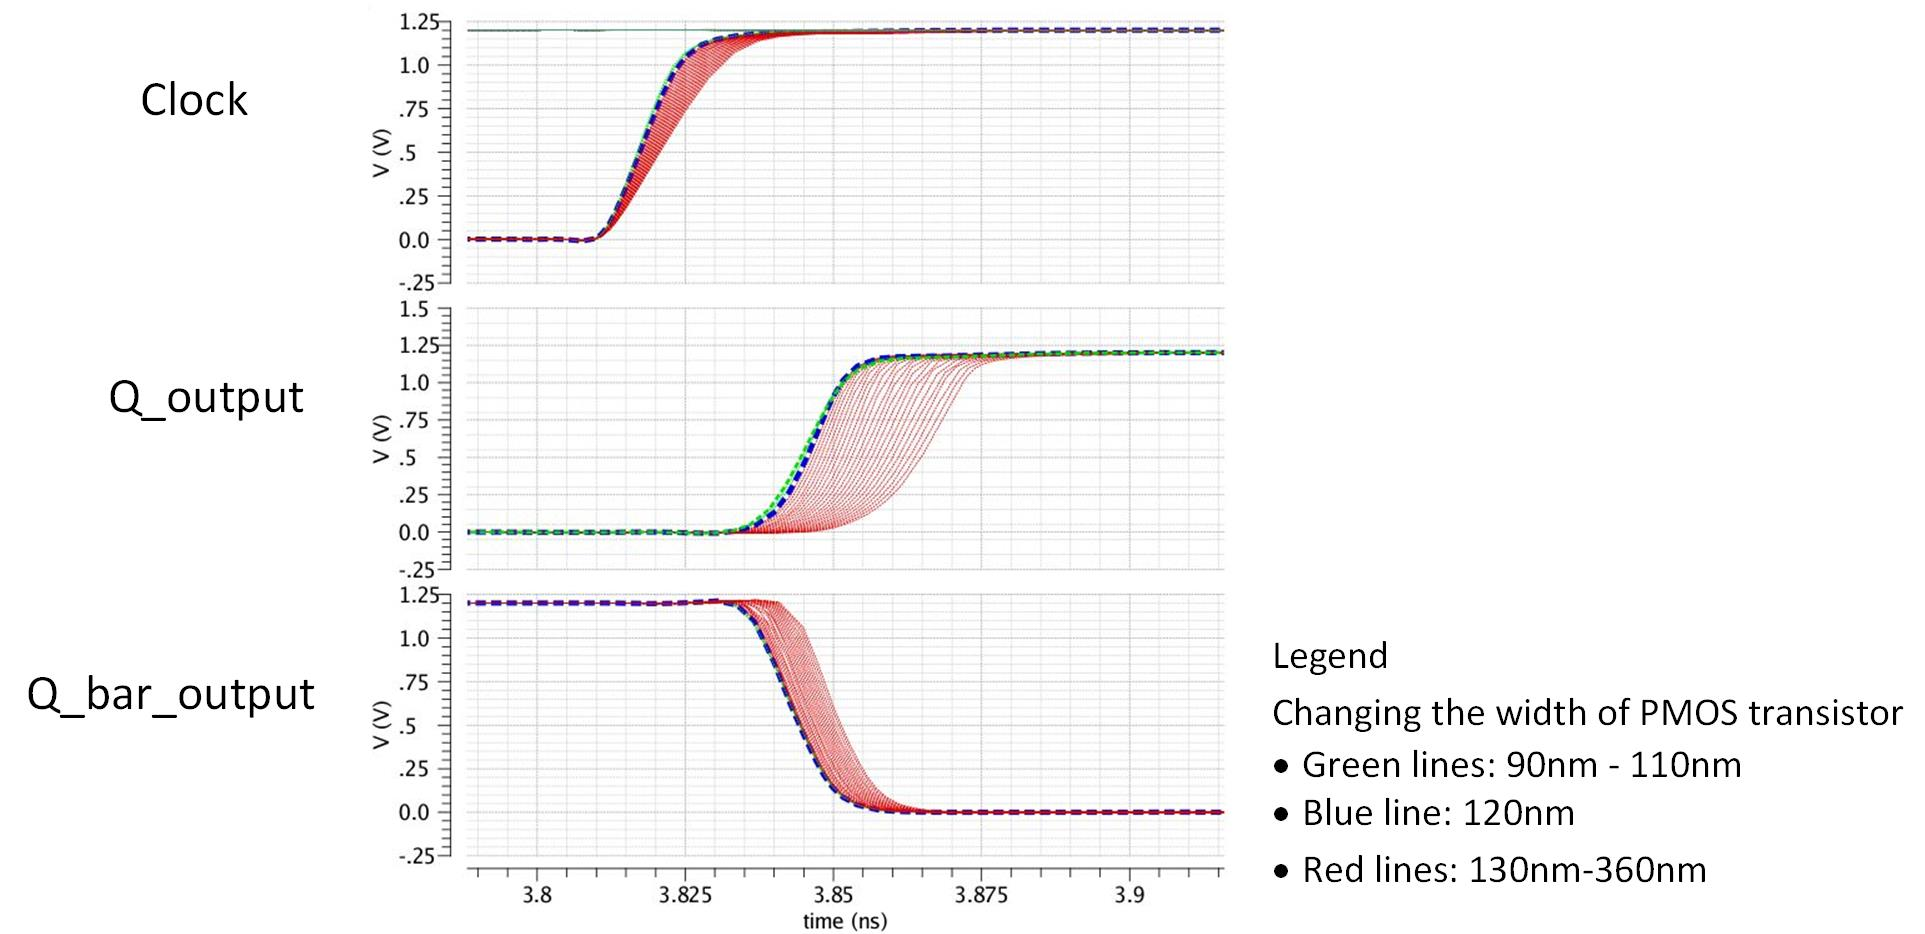
\includegraphics[width=0.5\textwidth]{Parameter_sweep_changing_w_low_to_high.jpg}
 \caption{A Parameter sweep of changing the width of the PMOS transistor when the data is high. The PMOS transistors of part 1,2 and 4 of~\ref{fig:D_flip_flop_schematic_figure} are part of the parameter sweep. The frequency of the clock is set to 1 GHz and the frequency of the data is set to 500MHz.}
 \label{fig:parametersweep_changing_w_low_to_high_figure}
\end{figure}

\begin{figure}[h]
 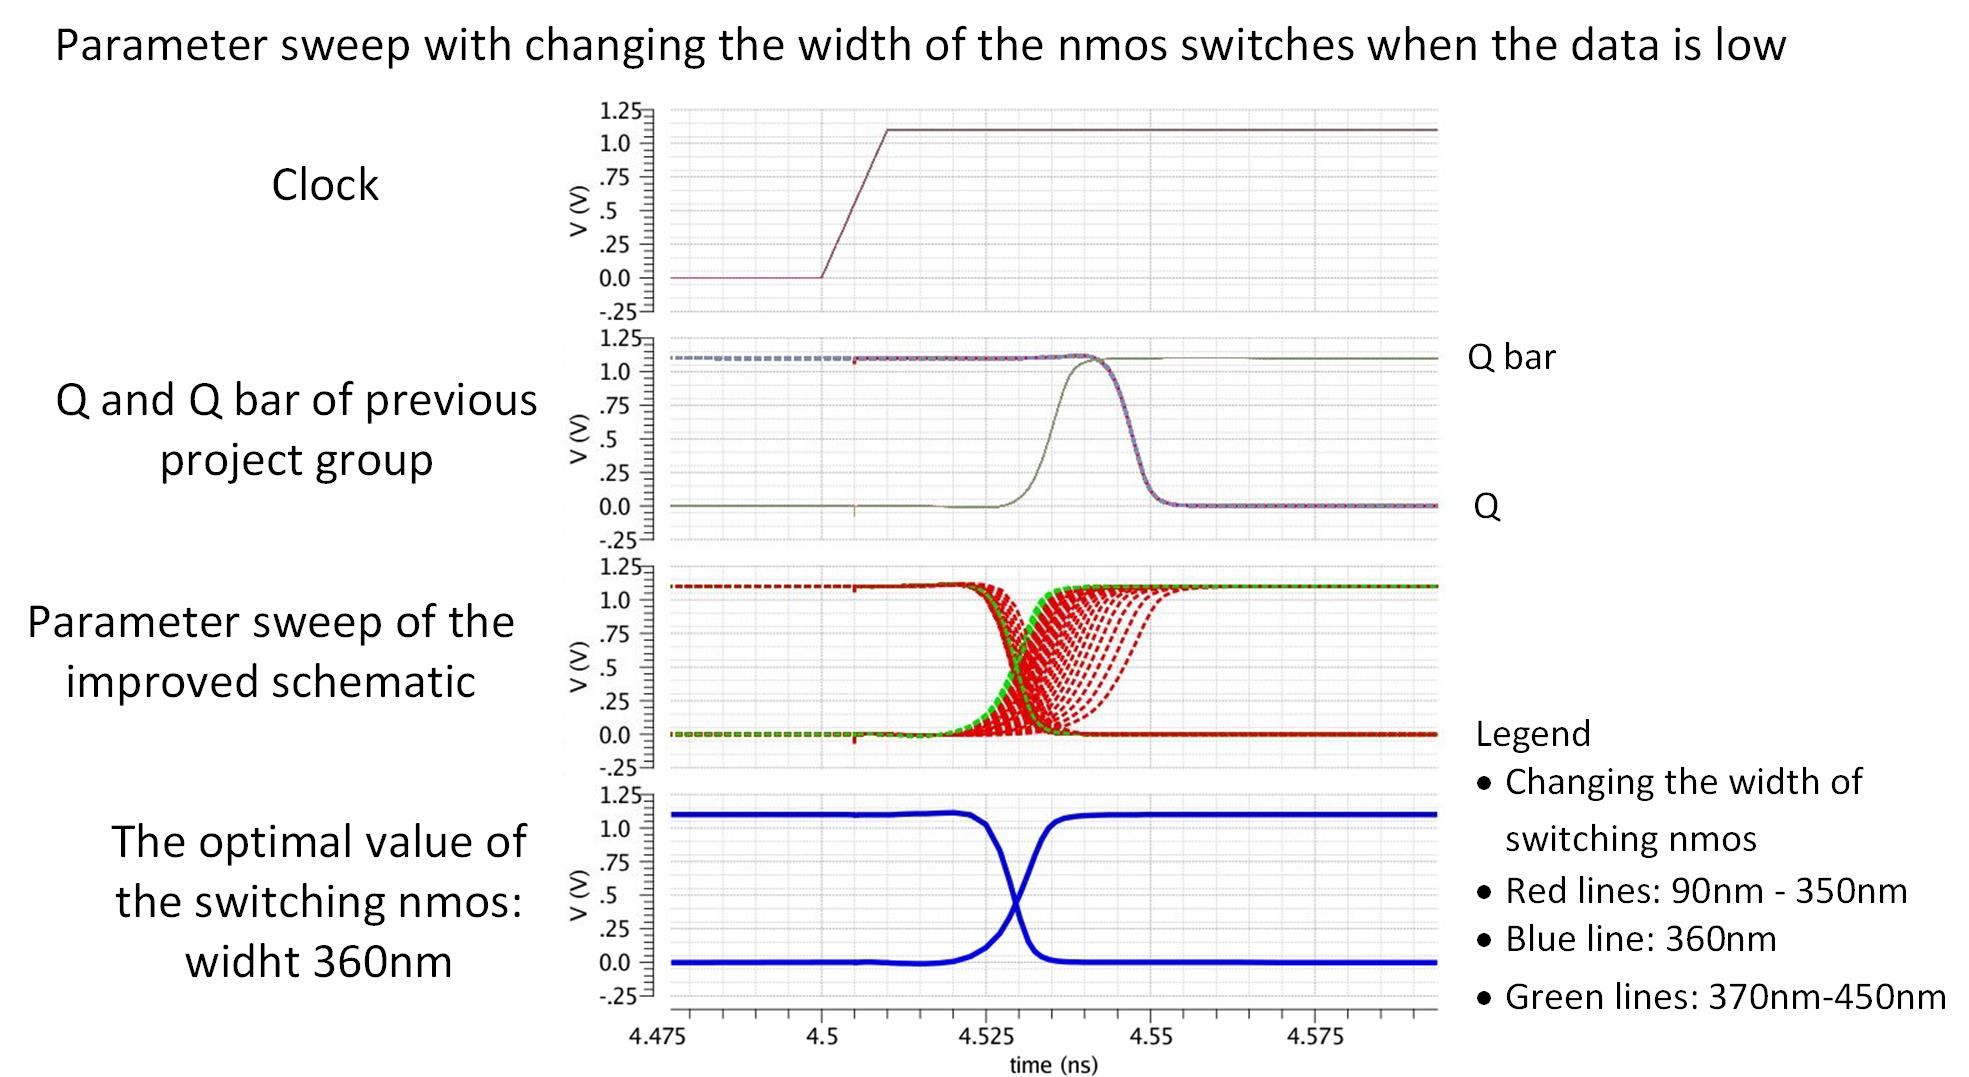
\includegraphics[width=0.5\textwidth]{Parameter_sweep_changing_w_of_the_swiching_nmos_high_to_low.jpg}
 \caption{Parameter sweep of changing the width of the NMOS transitor of part 3 in Fig.\ref{fig:D_flip_flop_schematic_figure} when the data is low.}
 \label{fig:Parameter_sweep_changing_w_of_the_swiching_nmos_high_to_low_figure}
\end{figure}

\begin{figure}[h]
 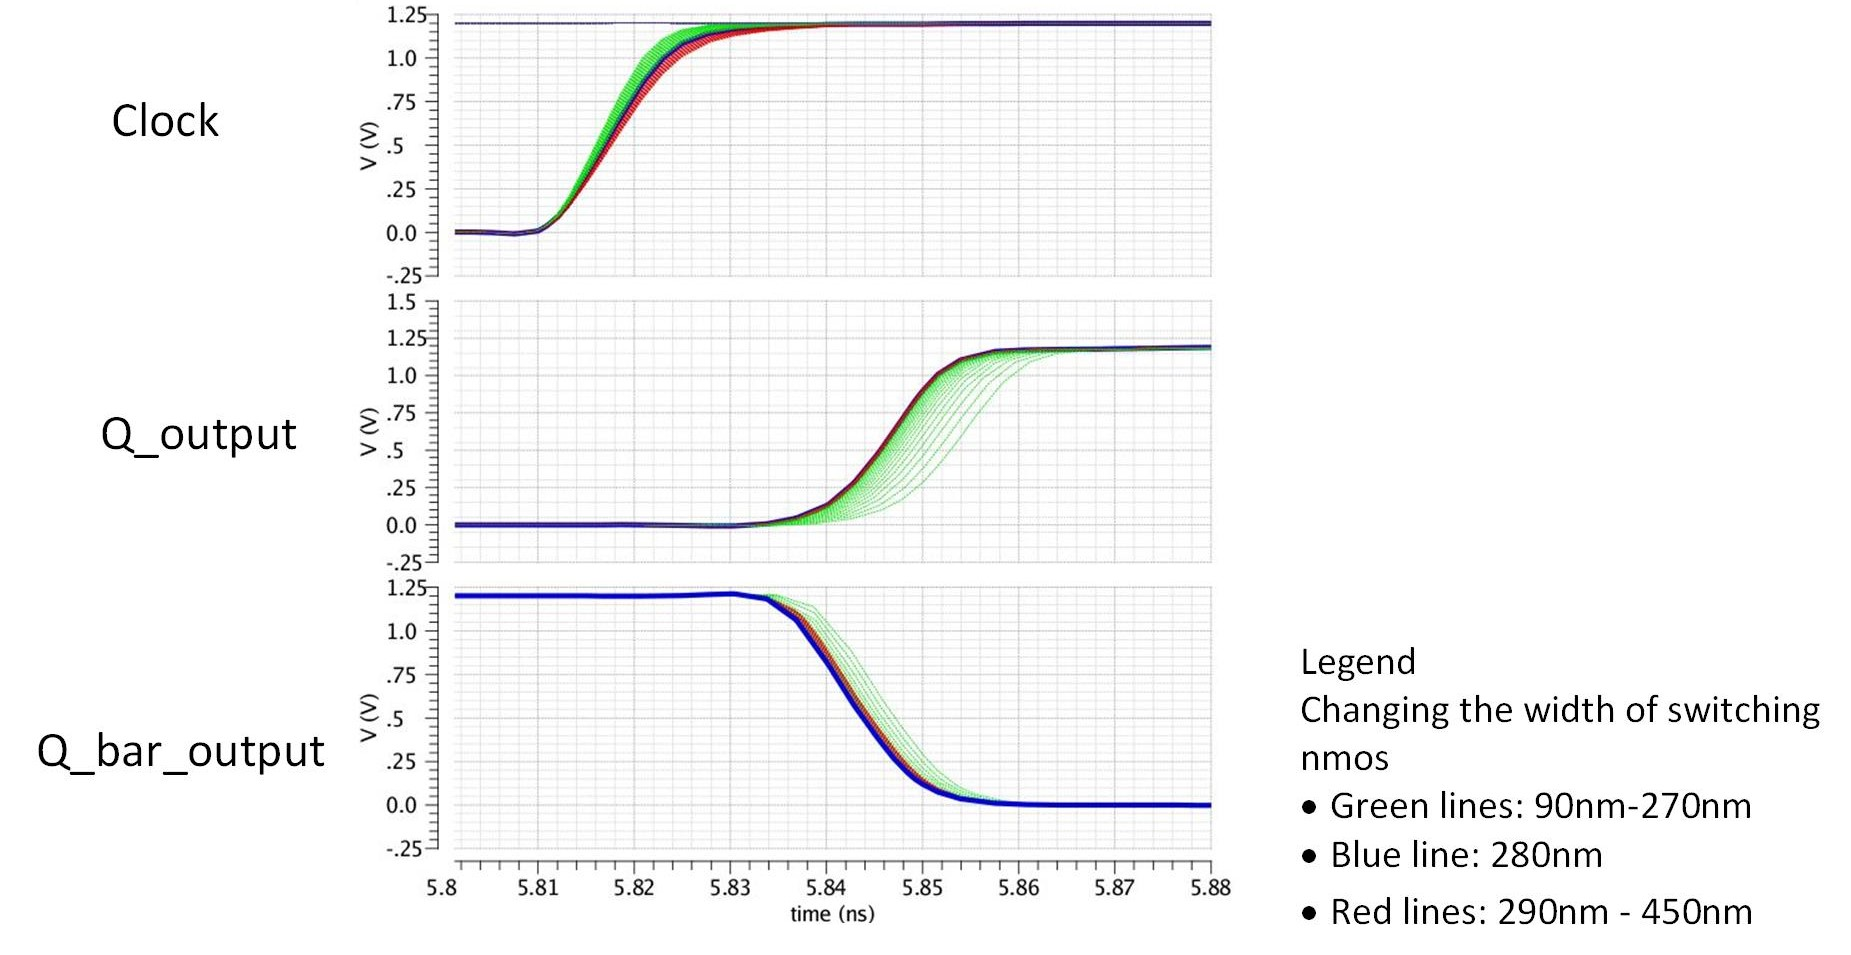
\includegraphics[width=0.5\textwidth]{Parameter_sweep_changing_w_of_the_swiching_nmos_low_to_high.jpg}
 \caption{Parameter sweep of changing the width of the NMOS transitor of part 3 in Fig.\ref{fig:D_flip_flop_schematic_figure} when the data is high.}
 \label{fig:Parameter_sweep_changing_w_of_the_swiching_nmos_low_to_high_figure}
\end{figure}

\begin{figure}[h]
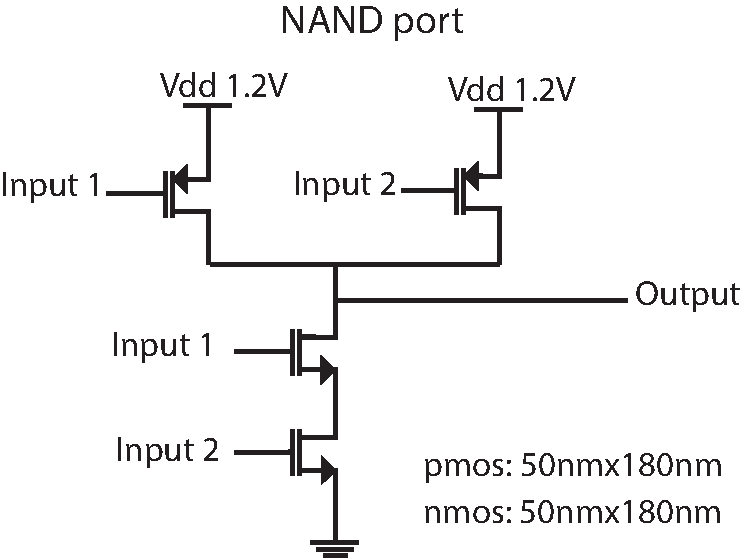
\includegraphics[width=0.4\textwidth]{NAND_schematic.pdf}
\caption{The schematic of the NAND gate.}
\label{fig:NAND_schematic_figure}
\end{figure}

\begin{figure}[h]
 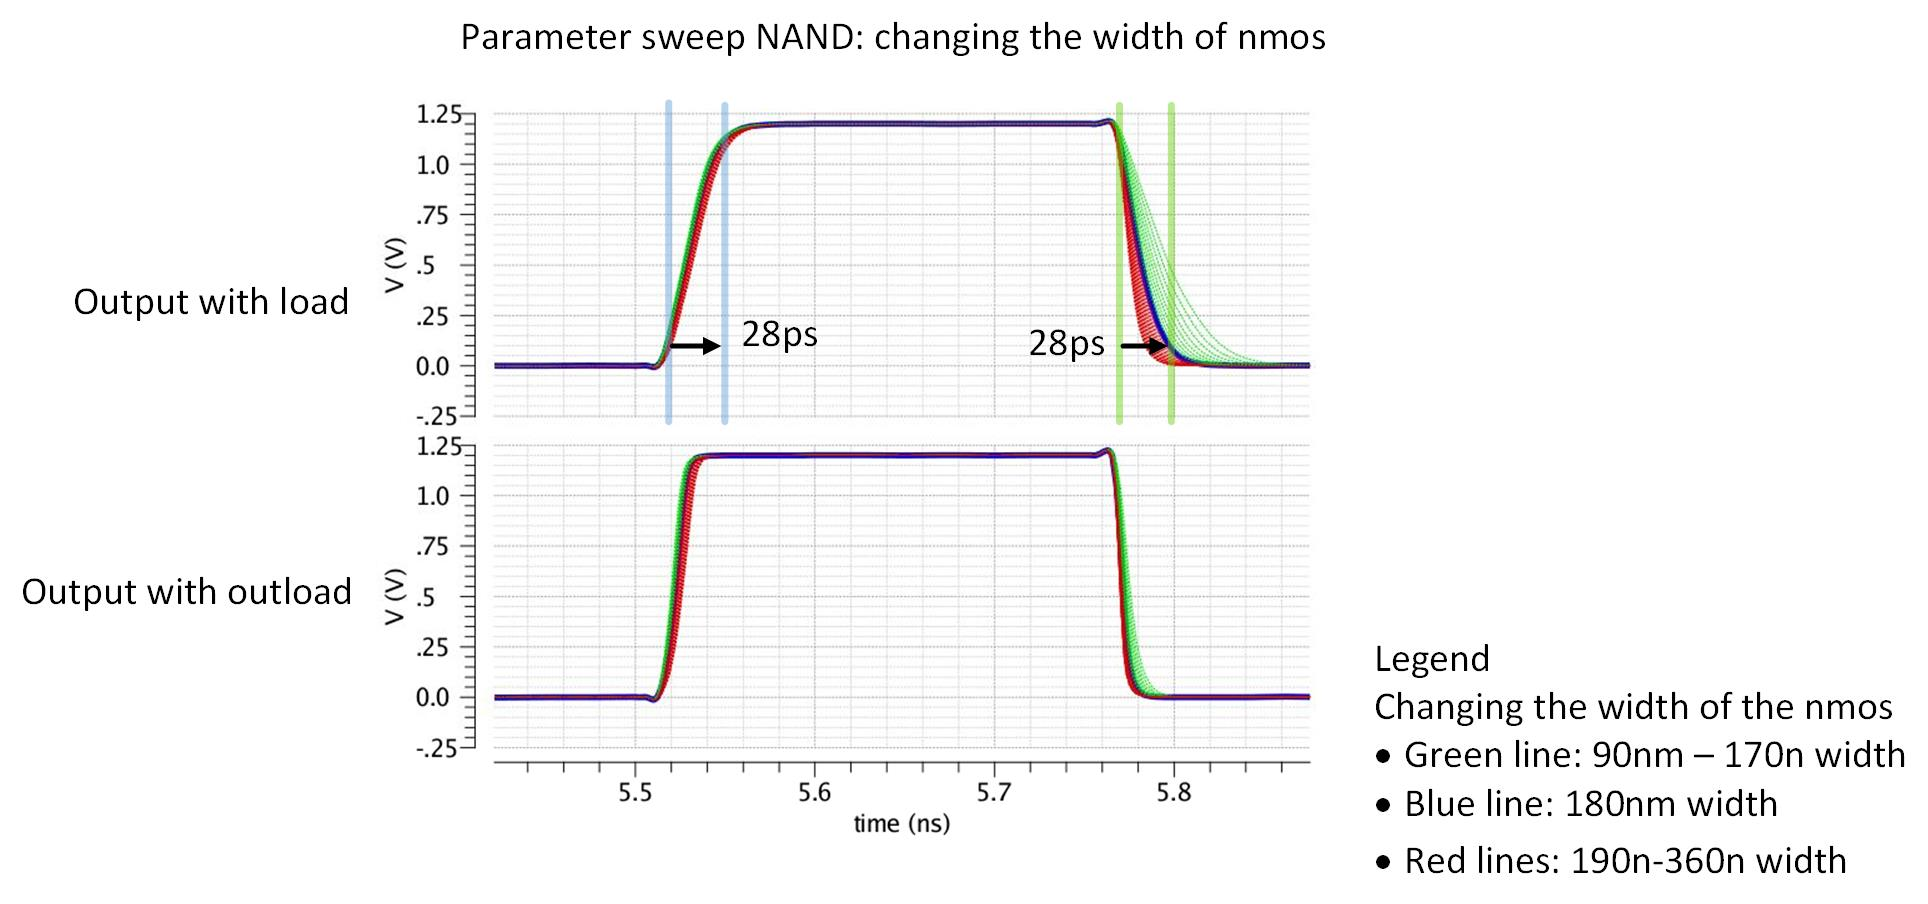
\includegraphics[width=0.5\textwidth]{NAND_nmos_sweep.jpg}
 \caption{Parameter sweep of changing the width NMOS transistor of the NAND gate.}
 \label{fig:NAND_nmos_sweep_figure}
\end{figure}

\begin{figure}[h]
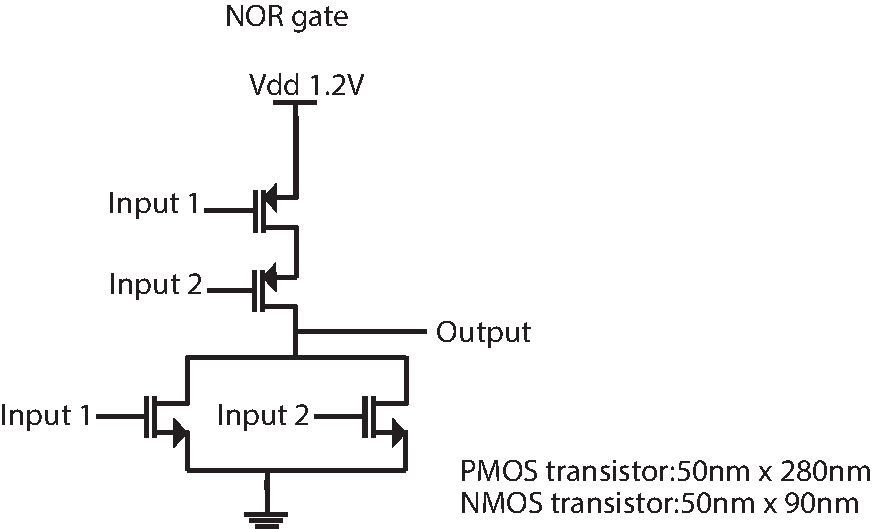
\includegraphics[width=0.35\textwidth]{NOR_schematic.pdf}
\caption{The schematic of the NOR gate.}
\label{fig:NOR_schematic_figure}
\end{figure}

\begin{figure}[h]
 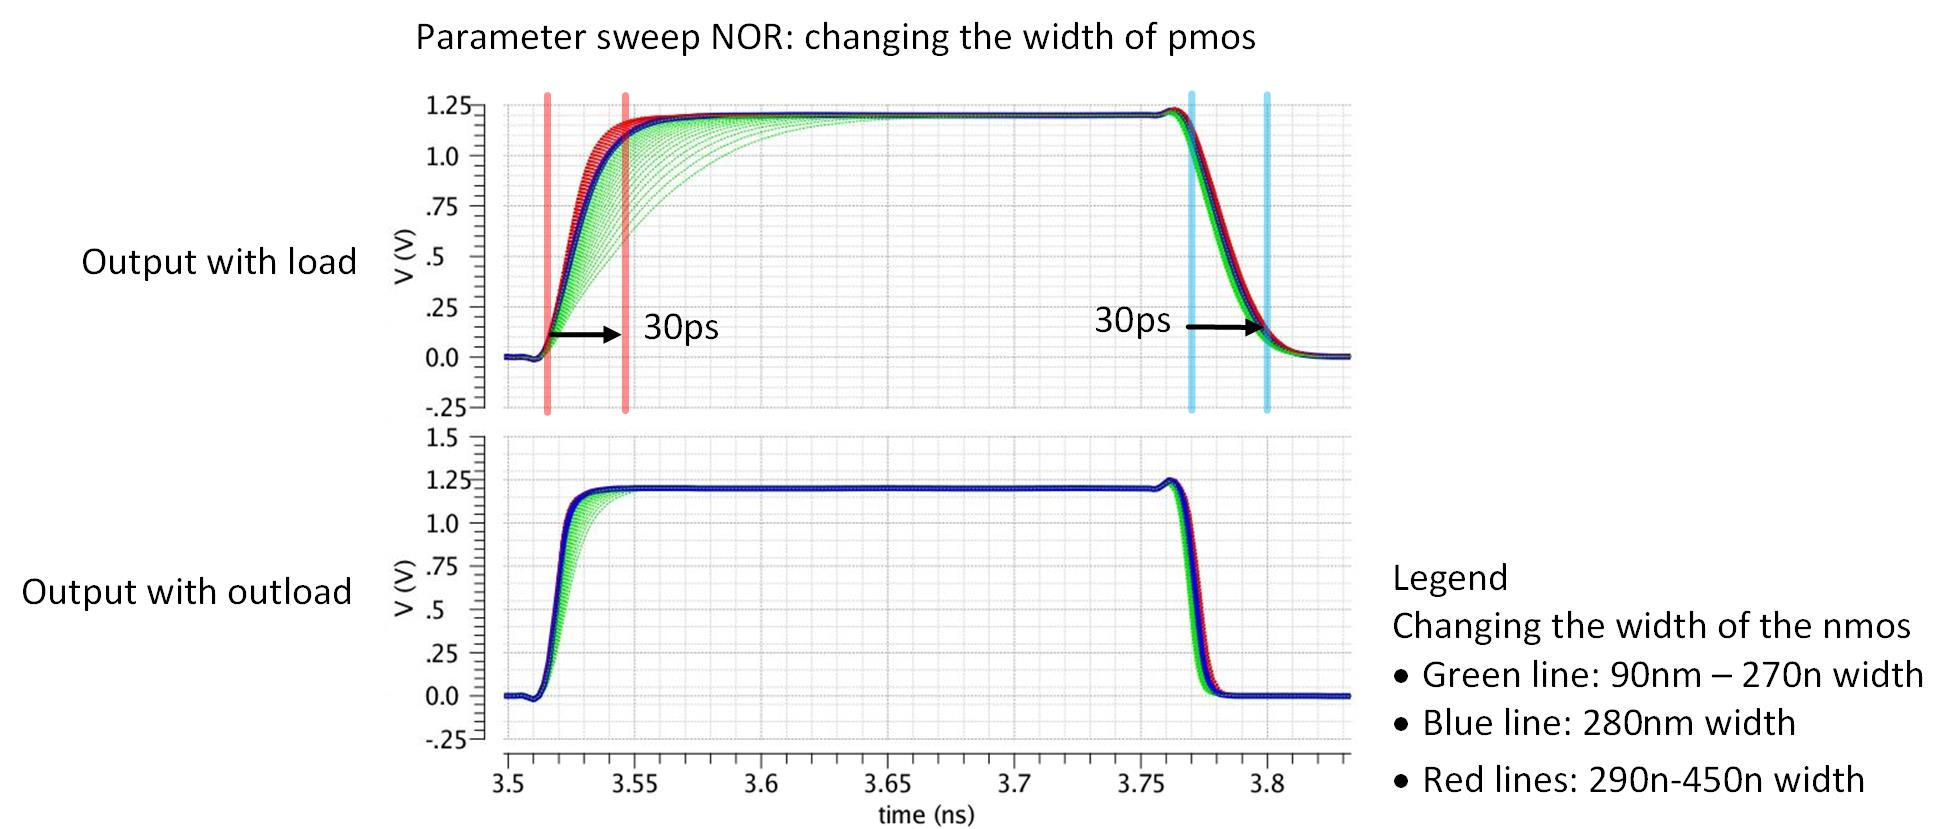
\includegraphics[width=0.5\textwidth]{NOR_pmos_sweep.jpg}
 \caption{Parameter sweep of changing the width NMOS transistor of the NOR gate.}
 \label{fig:NOR_pmos_sweep_figure}
\end{figure}

\begin{figure}[h]
 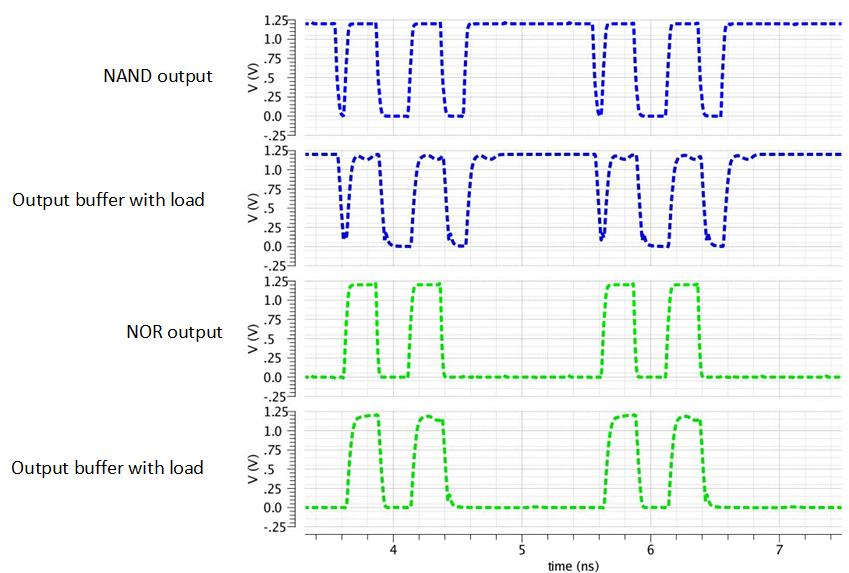
\includegraphics[width=0.5\textwidth]{Results_of_NAND_NOR_with_buffer.jpg}
 \caption{Results of the output of the NAND and NOR with a buffer.}
 \label{fig:Results_of_NAND_NOR_with_buffer_figure}
\end{figure}

\begin{table}[h!]
\caption{This table lists the dimensions of the transistors of the D flip-flops.}
\begin{tabular}{l||l|l}\arraybackslash
Transistor & Width(nm) & Length (nm) \\\hline\hline
M1 & 120 & 50\\\hline
M2 & 120 & 50\\\hline
M3 & 90 & 50\\\hline
M4 & 90 & 50\\\hline
M5 & 120 & 50\\\hline
M6 & 120 & 50\\\hline
M7 & 90 & 50\\\hline
M8 & 90 & 50\\\hline
M9 & 120 & 50\\\hline
M10 & 90 & 50\\\hline
M11 & 120 & 50\\\hline
M12 & 90 & 50\\\hline
M13 & 120 & 50\\\hline
M14 & 90 & 50\\\hline
M15 & 280 & 50\\\hline
M16 & 280 & 50\\\hline
M17 & 120 & 50\\\hline
M18 & 120 & 50\\\hline
M19 & 90 & 50\\\hline
M20 & 90 & 50\\\hline
M21 & 120 & 50\\\hline
M22 & 90 & 50\\\hline
M23 & 120 & 50\\\hline
M24 & 90 & 50\\\hline
M25 & 120 & 50\\\hline
M26 & 120 & 50\\\hline
M27 & 90 & 50\\\hline
M28 & 90 & 50\\\hline
M29 & 120 & 50\\\hline
M30 & 90 & 50\\\hline
M31 & 120 & 50\\\hline
M32 & 90 & 50
\end{tabular}
\label{Tab:D_flip-flop_transistor_sizes}
\end{table}

\begin{table}[h!]
\caption{This table lists the dimensions of the transistors in the levelshifter that drives the PMOS current sources.}
\begin{tabular}{l||l|l}\arraybackslash
Transistor & Width(um) & Length (nm) \\\hline\hline
M1 & 10 & 200\\\hline
M2 & 50 & 200\\\hline
M3 & 10 & 275\\\hline
M4 & 10 & 275\\\hline
M5 & 1.1 & 50\\\hline
M6 & 1.1 & 50
\end{tabular}
\label{Tab:Levelshifter_PMOS_sizes}
\end{table}

\begin{table}[h!]
\caption{This table lists the dimensions of the transistors in the levelshifter that drives the NMOS current sources.}
\begin{tabular}{l||l|l}\arraybackslash
Transistor & Width(um) & Length (nm) \\\hline\hline
M1 & 10 & 200\\\hline
M2 & 50 & 200\\\hline
M3 & 10 & 275\\\hline
M4 & 10 & 275\\\hline
M5 & 1.1 & 50\\\hline
M6 & 1.1 & 50\\\hline
M7 & 20 & 1400\\\hline
M8 & 25 & 200
\end{tabular}
\label{Tab:Levelshifter_NMOS_sizes}
\end{table}

\begin{figure}[h]
\begin{center}
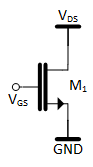
\includegraphics[width=0.1\textwidth]{NMOS_END_STAGE.png}
\caption{The circuit used to determine the required width of the transistor to sink 3.3mA. $V_{DS}$ is 2.4167V and $V_{GS}$ is 1.95V.}
\label{fig:NMOS_Width_Sweep}
\end{center}
\end{figure}

\begin{table}[h!]
\caption{This table describes which widths and lengths are used for which NMOS transistors. M1 is the MOSFET which is associated with the lowest current while M15 is associated with the highest current.}
\begin{tabular}{l||l|l}\arraybackslash
NMOS & Width(um) & Length (um) \\\hline\hline
M1 & 10.97 & 0.3\\\hline
M2 & 11.47 & 0.3\\\hline
M3 & 11.60 & 0.3\\\hline
M4 &  11.53 & 0.3\\\hline
M5 & 11.52 & 0.3\\\hline
M6 & 11.63 & 0.3\\\hline
M7 & 11.67 & 0.3\\\hline
M8 & 11.71 & 0.3\\\hline
M9 & 11.76 & 0.3\\\hline
M10 & 11.83 & 0.3\\\hline
M11 & 11.88 & 0.3\\\hline
M12 & 11.96 & 0.3\\\hline
M13 & 12.03 & 0.3\\\hline
M14 & 12.11 & 0.3\\\hline
M15 & 12.20 & 0.3
\end{tabular}
\label{Tab:NMOS}
\end{table}

\begin{table}
\caption{This table describes which widths and lengths are used for which PMOS transistors. M1 is the MOSFET which is associated with the lowest current while M15 is associated with the highest current.} 
\begin{tabular}{l||l|l}
PMOS & Width(um) & Length (um) \\\hline\hline
M1 & 56.23 & 0.3\\\hline
M2 & 57.25 & 0.3\\\hline
M3 & 57.63 & 0.3\\\hline
M4 & 57.84& 0.3\\\hline
M5 & 58.04 & 0.3\\\hline
M6 & 58.28 & 0.3\\\hline
M7 & 58.56 & 0.3\\\hline
M8 & 58.87 & 0.3\\\hline
M9 & 59.21 & 0.3\\\hline
M10 & 59.57 & 0.3\\\hline
M11 & 59.95 & 0.3\\\hline
M12 & 60.36 & 0.3\\\hline
M13 & 60.82 & 0.3\\\hline
M14 & 61.31 & 0.3\\\hline
M15 & 61.87 & 0.3
\end{tabular}
\label{Tab:PMOS}
\end{table}

\begin{figure}[h] 
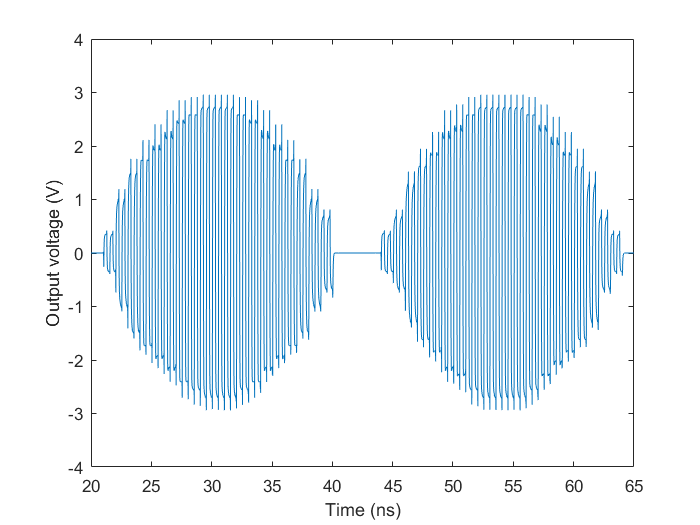
\includegraphics[width=0.5\textwidth]{Vout_one_tone.png}
\caption{42.97MHz single tone output voltage}
\label{fig:Vout_one_tone}
\end{figure}

\begin{figure}[h] 
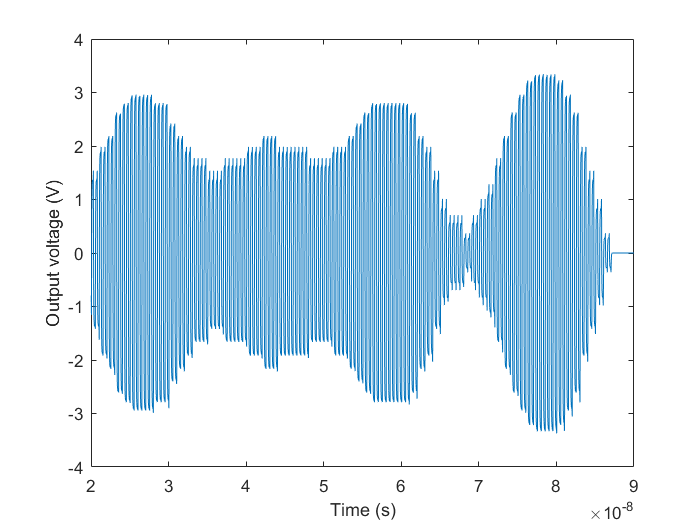
\includegraphics[width=0.5\textwidth]{Vout_two_tone.png}
\caption{42.97MHz and 54.69MHz two tone output voltage}
\label{fig:Vout_two_tone}
\end{figure}
\end{appendices}